\iffalse
\def\mytitle{MATRICES USING PYTHON}
\def\myauthor{P.kalyan}
\def\contact{kalyanpadyalaanirudh@gmail.com}
\def\mymodule{Future Wireless Communication (FWC)}
\documentclass[10pt, a4paper]{article}
\usepackage[a4paper,outer=1.5cm,inner=1.5cm,top=1.75cm,bottom=1.5cm]{geometry}
\twocolumn
\usepackage{graphicx}
\graphicspath{{./images/}}
\usepackage[colorlinks,linkcolor={black},citecolor={blue!80!black},urlcolor={blue!80!black}]{hyperref}
\usepackage[parfill]{parskip}
\usepackage{lmodern}
\usepackage{tikz}
	\usepackage{physics}
%\documentclass[tikz, border=2mm]{standalone}
\usepackage{karnaugh-map}
%\documentclass{article}
\usepackage{tabularx}
\usepackage{circuitikz}
\usetikzlibrary{calc}
\usepackage{amsmath}
\usepackage{amssymb}
\renewcommand*\familydefault{\sfdefault}
\usepackage{watermark}
\usepackage{lipsum}
\usepackage{xcolor}
\usepackage{listings}
\usepackage{float}
\usepackage{titlesec}
\providecommand{\mtx}[1]{\mathbf{#1}}
\titlespacing{\subsection}{1pt}{\parskip}{3pt}
\titlespacing{\subsubsection}{0pt}{\parskip}{-\parskip}
\titlespacing{\paragraph}{0pt}{\parskip}{\parskip}
\newcommand{\figuremacro}[5]{
    \begin{figure}[#1]
        \centering
        \includegraphics[width=#5\columnwidth]{#2}
        \caption[#3]{\textbf{#3}#4}
        \label{fig:#2}
    \end{figure}
}
\newcommand{\myvec}[1]{\ensuremath{\begin{pmatrix}#1\end{pmatrix}}}
\let\vec\mathbf
\lstset{
frame=single, 
breaklines=true,
columns=fullflexible
}

\thiswatermark{\centering \put(0,-90){
\includegraphics[scale=0.5]{iith}} }
\title{\mytitle}
\author{\myauthor\hspace{1em}\\\contact\\FWC22031\hspace{6.5em}IITH\hspace{0.5em}\mymodule\hspace{6em}ASSIGN-5}
\date{}
\begin{document}
	\maketitle
	\tableofcontents
   \section{Problem}
   \fi
   $ABC, ABD$ are 2 triangles on same base $AB$, if line segment $CD$ is bisected by $AB$ at $\vec{O}$, show that 
   \begin{align}
		\label{eq:9/9/3/4}
 ar (ABC) = ar (ABD)  
   \end{align}
	\begin{figure}[!h]
		\centering
 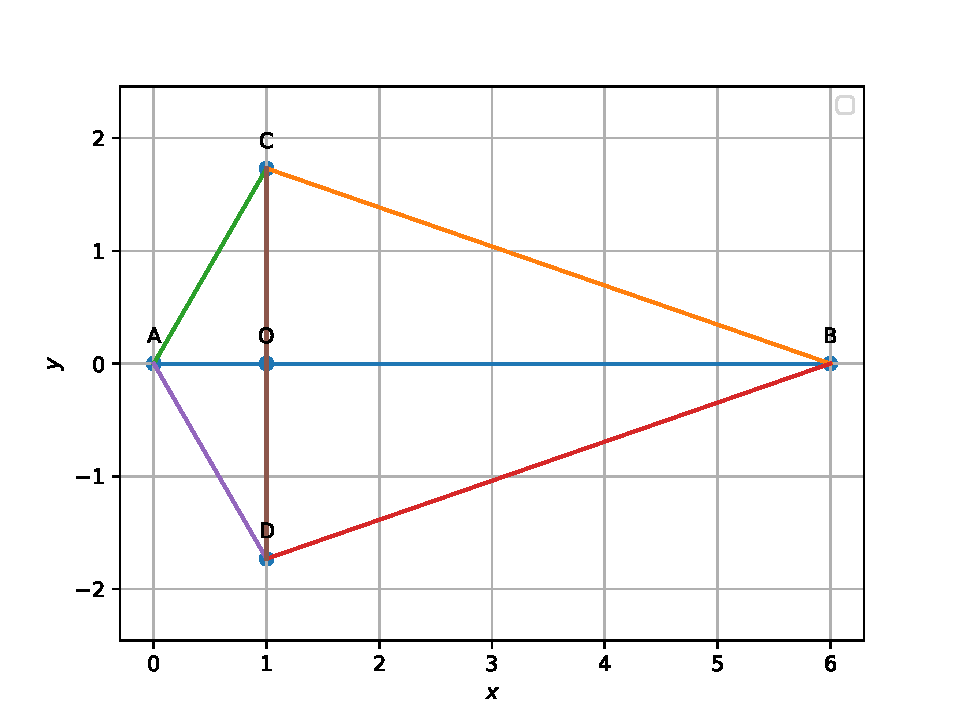
\includegraphics[width=\columnwidth]{chapters/9/9/3/4/figs/figa6.pdf}
		\caption{}
		\label{fig:9/9/3/4}
  	\end{figure}
	\begin{proof}
		See Fig. 
		\ref{fig:9/9/3/4}. $AO$ and $OB$ are medians of triangles $ADC$ and $BDC$. From 
Appendix	  \ref{prop:two-median-area}, 
		\eqref{eq:9/9/3/4} is trivial.
	\end{proof}


\iffalse

	    \includegraphics[scale=1.0]{}
   \section{Solution}
   \textbf{Theory:}\\
In 2 triangles with same base and linesegment cd is bisected at o  
\textbf{To Prove:} Ar(ABC)=Ar(ABD) \\
\textbf{Theorem} : Two triangles on the same base (or equal bases) and having the equal heights are equal in area.
\begin{center}
$\therefore$ Ar($\Delta$ ABC)=Ar($\Delta$ ABD)......(1)\\
Hence, Proved    
\end{center}


\
\textbf{termux commands :}
\begin{lstlisting}
python3 matrix.py
\end{lstlisting}


The input parameters for this construction are 
\begin{center}
\begin{tabular}{|c|c|c|}
	\hline
	\textbf{Symbol}&\textbf{Value}&\textbf{Description}\\
	\hline
	k1&4&length of CD\\
	\hline
	k2&6&length of AB\\
	\hline
 
	\hline
	O&$\
	\begin{pmatrix}
		0 \\
		0 \\
	\end{pmatrix}$%
	&Point O\\
	
	\hline
\end{tabular}
\end{center}
\textbf{To Prove:} Ar(ABC)=Ar(ABD)
  %	\begin{align}
	%		\vec{C} &= \myvec{0 \\ 0}, \vec{E}=\myvec{-5 \\ 3}\\
	%			\vec{F} &= \myvec{3 \\ 0}, \vec{D}=\myvec{-3 \\ 0}
	%	\end{align}
		\begin{center}
	a=A-B\\
	b=C-B\\
	c=B-D\\
	Area of the $\Delta$ABC is given by \\
Ar($\Delta$ABC) =$\frac{1}{2}$$\norm{\vec{a}\times\vec{b}}$............(2)\\
    b=C-B\\
	c=B-D\\
		Area of the $\Delta$ABD is given by \\
 Ar($\Delta$ABD) =$\frac{1}{2}$$\norm{\vec{c}\times\vec{d}}$...............(3)
	\end{center}
	
	\begin{center}
$\therefore$ Ar(ABC)=Ar(ABD)........(4)\\
	\end{center}
The below python code realizes the above construction:	
\begin{lstlisting}
https://github.com/anirudhkalyan/fwc
\end{lstlisting}
 \section{Construction}
 	\begin{center}
  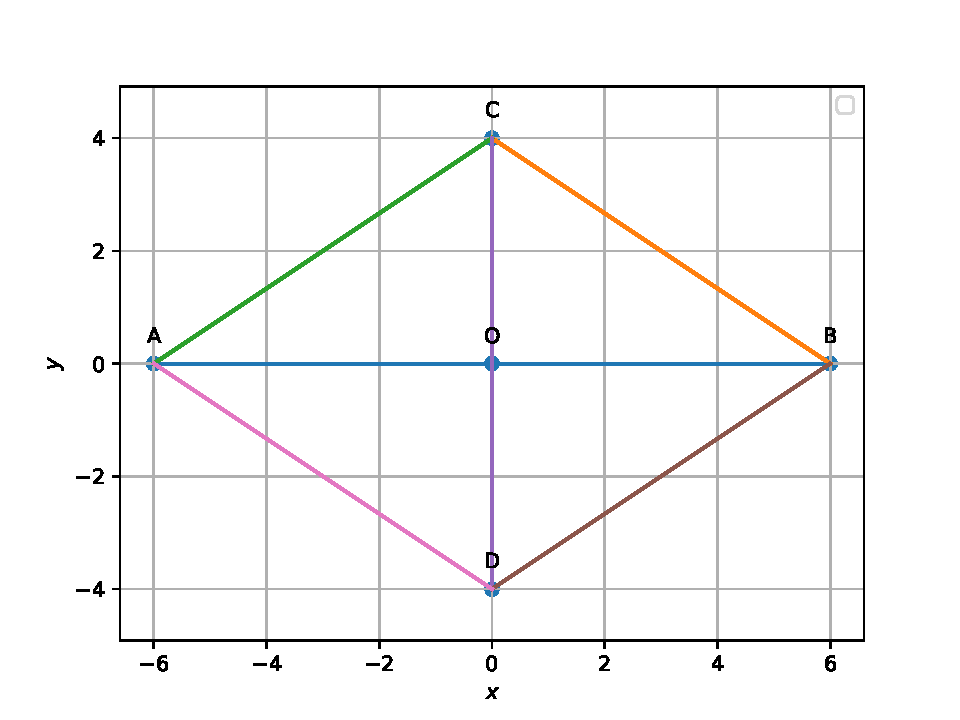
\includegraphics[scale=0.49]{figsa1.pdf}
  
  Figure of construction
  	\end{center}
  	  
\bibliographystyle{ieeetr}
\end{document}
\fi
